\documentclass{article}

\usepackage[margin=1in]{geometry}
\usepackage{graphicx} % Allow image/pdf includes
\usepackage{extramarks} % Extra header marks (continued on next page)
\usepackage{amsmath} % Math enhancements
\usepackage{amsthm} % Theorem typesetting
\usepackage{amssymb} % Extended symbol collection
\usepackage{tikz} % Graphical element creation
\usetikzlibrary{automata,positioning}
\usepackage{algpseudocode} % Algorithm layout
\usepackage{enumitem} % Enumerate (lists)
\usepackage{ragged2e} % Alternative alignment
\usepackage{gensymb} % Generic symbols (degree, etc)
\usepackage{empheq} % Allow \boxed around \begin{empheq}
\usepackage{color,soul} % Highlighting
\usepackage{booktabs} % Enhanced table creation
\usepackage{multirow} % Table multi row
\usepackage{mathtools} % Math enhancements
\usepackage{bm} % Bold math
\usepackage[mathscr]{euscript} % Script variables
\usepackage{cancel} % Cancel through text
\usepackage{color,soul} % Highlighting
\usepackage{mathtools}
\usepackage{multirow}
\usepackage{mathrsfs}
\usepackage{physics}
\usepackage{gensymb}
\usepackage{siunitx}
\usepackage{subcaption}
\usepackage[]{algorithm2e}
\usepackage{float}
\usepackage[cache=false]{minted}
\renewcommand{\MintedPygmentize}{/Users/loganharbour/miniconda/bin/pygmentize}
\usepackage[scaled]{beramono}
\usepackage[T1]{fontenc}
\usepackage{diagbox}

\setlength\parindent{0pt} % No indents
\setlength{\parskip}{1em} % Paragraph skip

\newcommand{\vx}{\mathbf{x}} % x vector
\newcommand{\vy}{\mathbf{y}} % x vector

\newcommand{\pageTitle}{MEEN 644 - Final Exam}
\newcommand{\pageAuthor}{Logan Harbour}

\begin{document}

\title{\LARGE \textbf{\pageTitle} \vspace{-0.3cm}}
\author{\large \pageAuthor}
\date{\vspace{-0.6cm} \large \today \vspace{-0.4cm}}

\maketitle

\section{Problem statement}

\begin{center}
	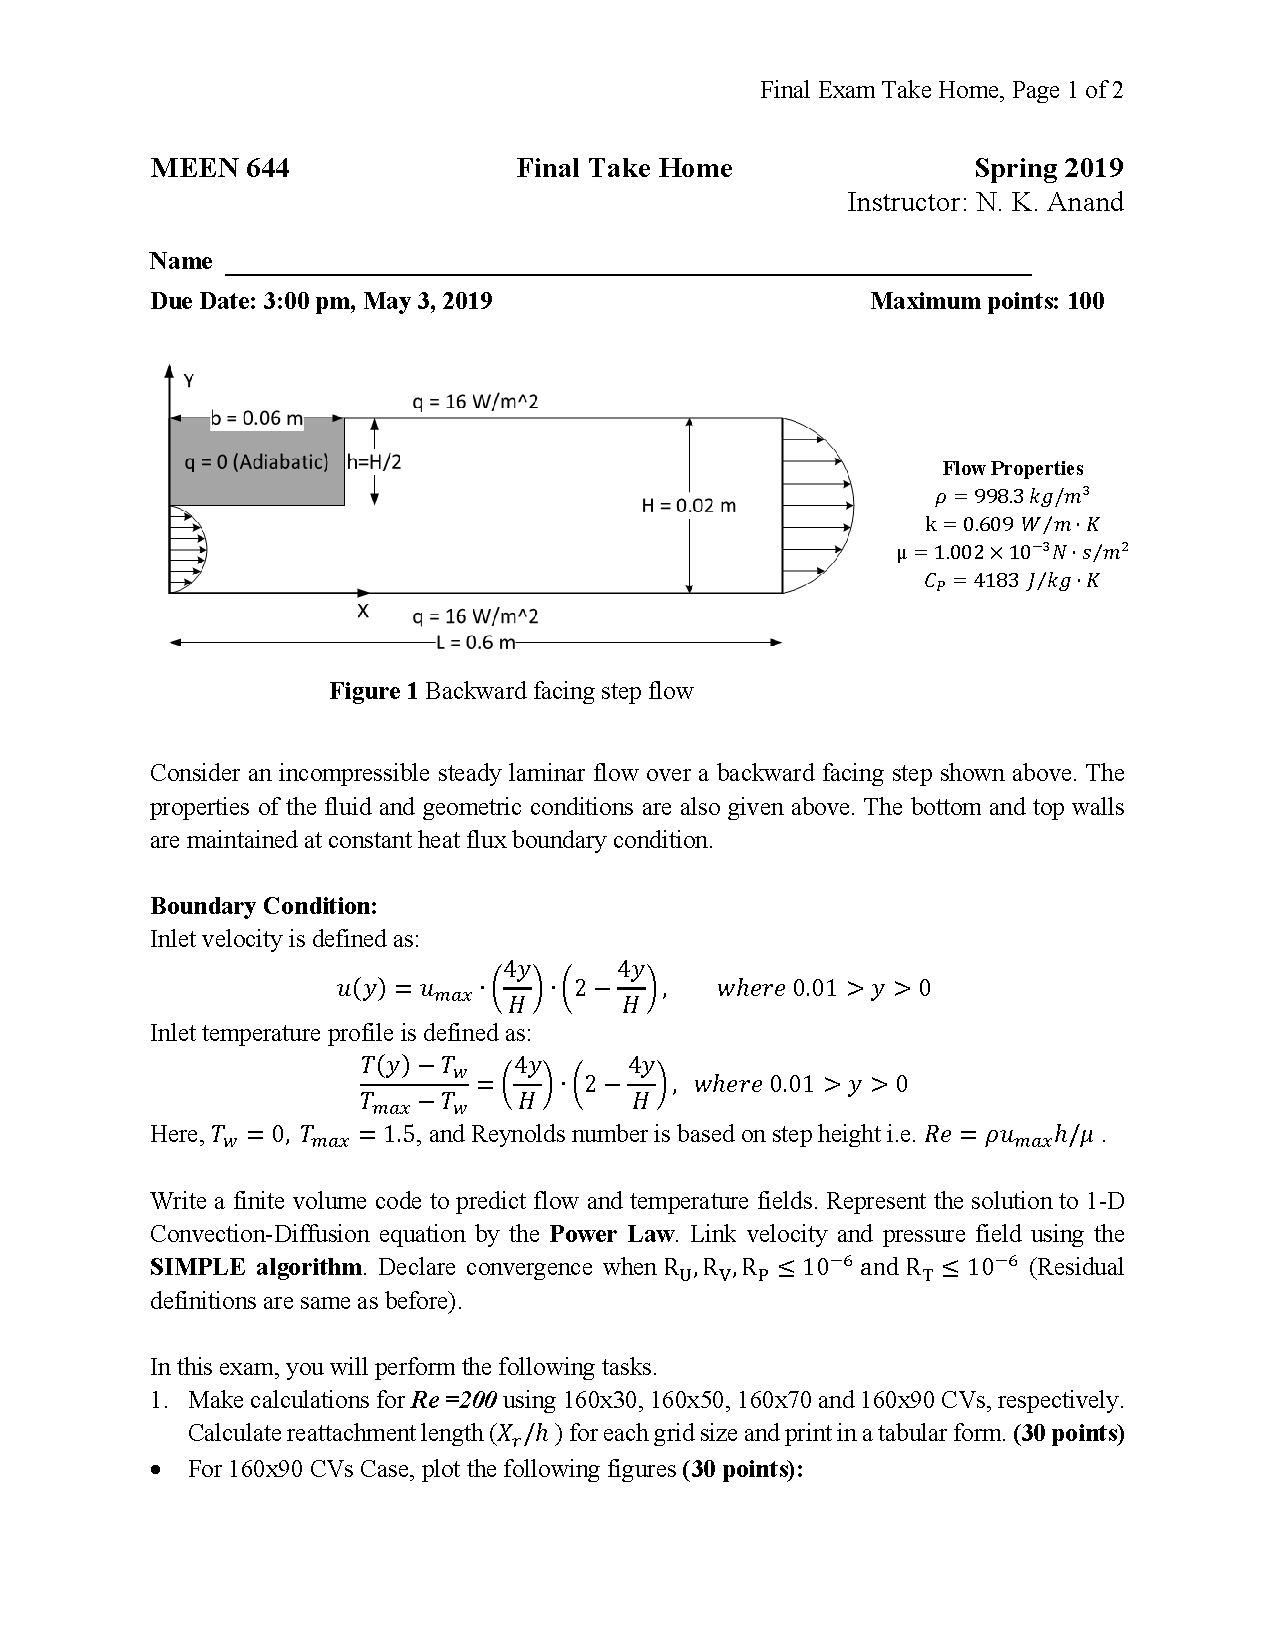
\includegraphics[trim={2.8cm 16.8cm 2.5cm 6cm},clip,page=1,scale=0.8]{../doc/final.pdf}
\end{center}

Consider an incompressible steady laminar flow over a backward facing step shown above. The properties of the fluid and geometric conditions are also given above. The bottom and top walls are maintained at constant heat flux boundary condition.

The inlet velocity is defined as
\[
	u(y) = u_\mathrm{max} \left(\frac{4y}{H}\right) \left(2 - \frac{4y}{H}\right)\,, \quad \text{where } 0.01 > y > 0\,,
\]
and the inlet temperature profile is defined as
\[
	\frac{T(y) - T_\mathrm{w}}{T_\mathrm{max} - T_\mathrm{w}} = \left(\frac{4y}{H}\right) \left(2 - \frac{4y}{H}\right)\,, \quad \text{where } 0.01 > y > 0\,,
\]
where $T_\mathrm{w} = 0, T_\mathrm{max} = 1.5$, and the Reynolds number is based on step height, i.e., Re $=\rho u_\mathrm{max} h/\mu$.

Write a finite volume code to predict flow and temperature fields. Represent the solution to the 1-D convection-diffusion equation by the Power Law. Link velocity and pressure fields using the SIMPLE algorithm. Declare convergence when $R_u, R_v, R_p,$ and $R_T \leq 10^{-6}$.

In this exam, the following tasks are performed:
\begin{enumerate}
	\item \textbf{(60 points)} Make calculations using Re = 200 using 160$\times$30, 160$\times$50, 160$\times$70, and 160$\times$90 CVs, respectively. Calculate reattachment length for each grid size and print in a tabular form. For the 160$\times$90 CV case, plot the following figures:
	\begin{enumerate}[label=(\alph*)]
		\item Plot the temperature profile at $(x - b)/H = 6, 12$ and $24$.
		\item Plot both upper and lower wall temperature along the wall length.
		\item Plot Nusselt number for both upper and lower wall along the channel length.
	\end{enumerate}
	\item \textbf{(40 points)} Calculate reattachment length for Re $= 100, 300,$ and $400$. Use 160$\times$70 CVs. Compare your results with the experimental data in the reference. Print your comparison results in tabular form. For each Reynolds number, plot the $u$ and $v$-velocity profiles at $(x - b)/H = 6, 12,$ and $24$.
\end{enumerate}

\section{Preliminaries}

See Homeworks 4 and 5 for discussion of the solving methodology. The only difference between the methods used in said two homeworks was the implementation of variable material properties for $k$ and $\mu$. At initialization, these properties were set at the CV centroids as
\begin{align}
	k_p^{T_{i,j}} & =
	\begin{cases}
		10^{-99} \text{~W/m}\cdot\text{k} & x^{T_{i,j}} \leq b \quad \text{and} \quad y^{T_{i,j}} \geq h\ \\
		0.609 \text{~W/m}\cdot\text{k} & \text{otherwise}
	\end{cases}\,, \\
	\mu_p^{u_{i,j}} & =
	\begin{cases}
		10^{99} \text{~N}\cdot\text{s/m}^2 & x^{u_{i,j}} \leq b \quad \text{and} \quad y^{u_{i,j}} \geq h\ \\
		1.002 \times 10^{-3} \text{~N}\cdot\text{s/m}^2 & \text{otherwise}
	\end{cases}\,,\\
	\mu_p^{v_{i,j}} & =
	\begin{cases}
		10^{99} \text{~N}\cdot\text{s/m}^2 & x^{v_{i,j}} \leq b \quad \text{and} \quad y^{v_{i,j}} \geq h\ \\
		1.002 \times 10^{-3} \text{~N}\cdot\text{s/m}^2 & \text{otherwise}
	\end{cases}\,,
\end{align}
where $x^{\phi_{i,j}}$ represents the $x$-position of node $\phi_{i,j}$, and $y^{\phi_{i,j}}$ represents the $y$-position of node $\phi_{i,j}$.

The harmonic mean is then utilized to obtain the material properties at the CV edges. This is arbitrarily defined for material property $m$ of variable $\phi$ as
\begin{align}
	m_n^{\phi_{i,j}} & = \frac{2 m_p^{\phi_{i,j}} m_p^{\phi_{i,j+1}}}{m_p^{\phi_{i,j}} + m_p^{\phi_{i,j+1}}}\,,\\
	m_e^{\phi_{i,j}} & = \frac{2 m_p^{\phi_{i,j}} m_p^{\phi_{i+1,j}}}{m_p^{\phi_{i,j}} + m_p^{\phi_{i+1,j}}}\,,\\
	m_s^{\phi_{i,j}} & = \frac{2 m_p^{\phi_{i,j}} m_p^{\phi_{i,j-1}}}{m_p^{\phi_{i,j}} + m_p^{\phi_{i,j-1}}}\,,\\
	m_w^{\phi_{i,j}} & = \frac{2 m_p^{\phi_{i,j}} m_p^{\phi_{i-1,j}}}{m_p^{\phi_{i,j}} + m_p^{\phi_{i-1,j}}}\,.
\end{align}

The method of an arbitrarily large $\mu$ and arbitrarily small $k$ within the step was utilize to implement the solid-fluid interface.

\section{Results}

For all the results that follow, the following experimental correlation from Goldstein is used as the ``experimental'' comparison, given that the experimental results are not given for a specific Re:
\[
	x_r = h \times (2.13 + 0.021~\text{Re})\,.
\]

\subsection{Problem 1: Re = 200}

The results requested follow in Table 1 and Figures 1, 2, and 3.

\def\arraystretch{1.3}
\begin{table}[H]
	\small
	\centering
	\caption{Comparison of reattachment lengths for each grid size with Re = 200.}
	\vspace{0.2cm}
	\begin{tabular}{c|c|c}
		Grid size & Numerical & Experimental \\
		\hline
		$160\times30$ & 0.0592 & \multirow{4}{*}{0.0633} \\
		$160\times50$ & 0.0597 & \\
		$160\times70$ & 0.0598 & \\
		$160\times90$ & 0.0598 & \\
	\end{tabular}
	\label{table:b-temps}
\end{table}

\begin{figure}[H]
	\centering
	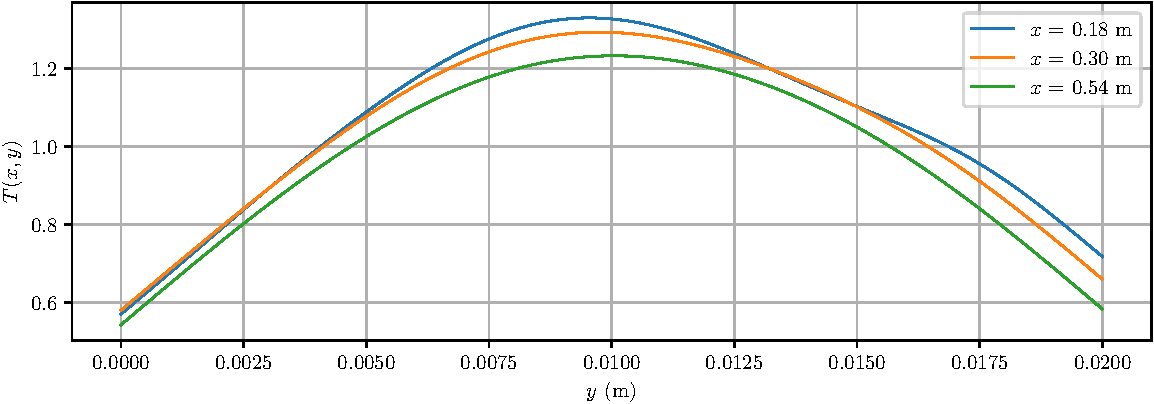
\includegraphics[width=0.9\linewidth]{../results/1a_Ty}
	\caption{The $y$-temperature profile at various points in the channel for the 160$\times$90 CV case with Re = 200.}
	\label{fig:1a_Ty}
\end{figure}

\begin{figure}[H]
	\centering
	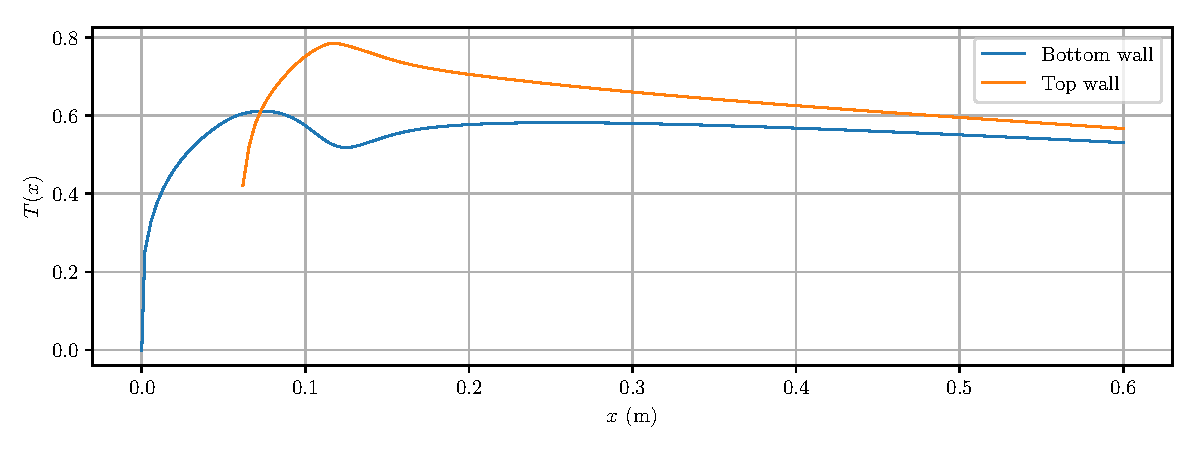
\includegraphics[width=0.9\linewidth]{../results/1b_Twall}
	\caption{The wall temperature profiles for the 160$\times$90 CV case with Re = 200.}
	\label{fig:1b_Twall}
\end{figure}

\begin{figure}[H]
	\centering
	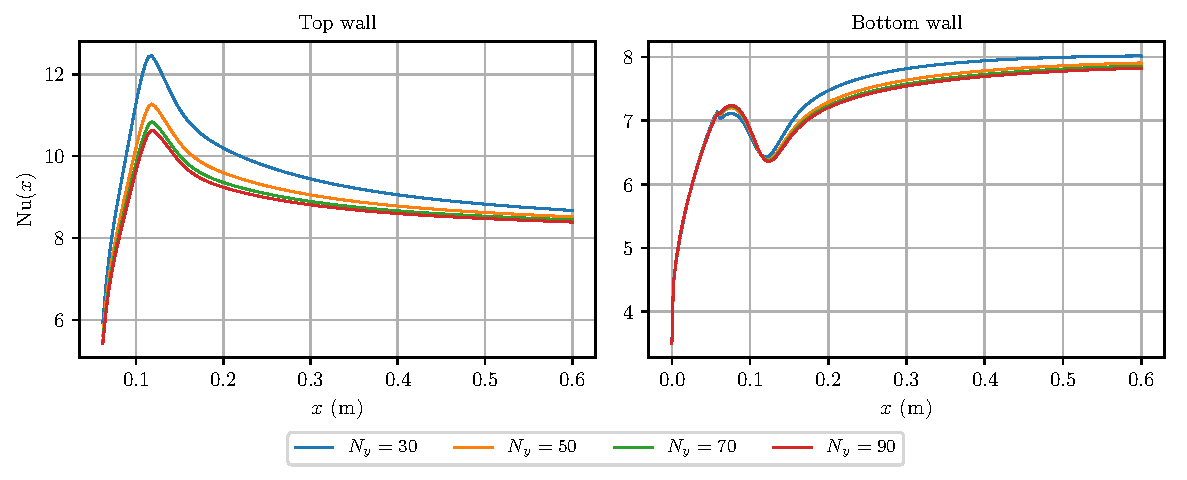
\includegraphics[width=0.9\linewidth]{../results/1c_Nu}
	\caption{The wall Nusselt numbers for the 160$\times$90 CV case with Re = 200.}
	\label{fig:1c_Nu}
\end{figure}

\subsection{Problem 2: Re = 100, 300, and 400}

The results requested follow in Table 2 and Figures 4 and 5.

\def\arraystretch{1.3}
\begin{table}[H]
	\small
	\centering
	\caption{Comparison of reattachment lengths with $160 \times 70$ CVs.}
	\vspace{0.2cm}
	\begin{tabular}{c|c|c}
		Re & Numerical & Experimental \\
		\hline
		100 & 0.0358 & 0.0423 \\
		300 & 0.0773 & 0.0843 \\
		400 & 0.0829 & 0.1053 \\
	\end{tabular}
	\label{table:b-temps}
\end{table}

\begin{figure}[H]
	\centering
	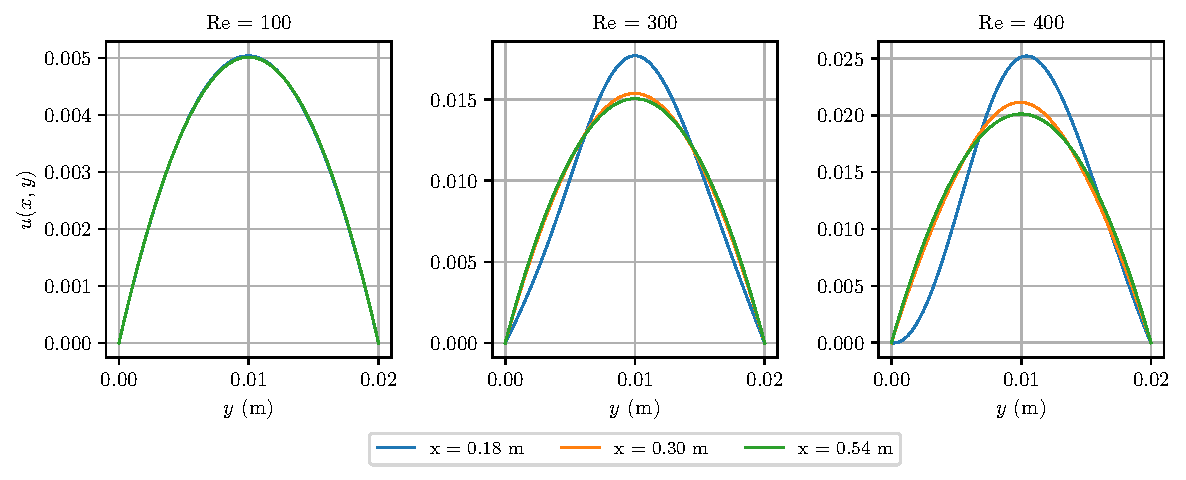
\includegraphics[width=0.9\linewidth]{../results/2_u}
	\caption{The $u$-velocity profiles at various points in the channel for the 160$\times$70 CV case.}
	\label{fig:2_u}
\end{figure}

\begin{figure}[H]
	\centering
	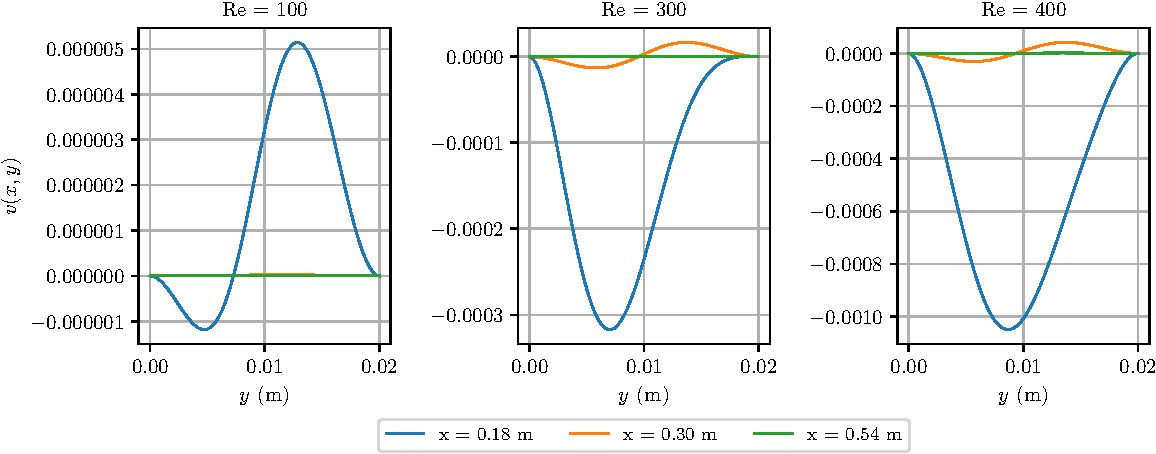
\includegraphics[width=0.9\linewidth]{../results/2_v}
	\caption{The $v$-velocity profiles at various points in the channel for the 160$\times$70 CV case.}
	\label{fig:2_v}
\end{figure}


\section*{Code listing}

For the implementation, we have the following files:
\begin{itemize}
	\item \texttt{Makefile} -- Allows for compiling the c++ project with \texttt{make}.
	\item \texttt{final.cpp} -- Contains the \texttt{main()} function that is required by C that runs the cases requested in this problem set.
	\item \texttt{Problem.h} -- Contains the header for the \texttt{Problem} class which is the main driver for a \texttt{Flow2D::Problem}.
	\item \texttt{Variable.h} -- Contains the \texttt{Flow2D::Variable} class, which is a storage container for a single variable (i.e., $u$).
	\item \texttt{Problem.cpp} -- Contains the \texttt{run()} functions that executes a \texttt{Problem}.
	\item \texttt{Problem\_coefficients.cpp} -- Contains the functions for solving coefficients in a \texttt{Problem}.
	\item \texttt{Problem\_corrections.cpp} -- Contains the functions for correcting solutions in a \texttt{Problem}.
	\item \texttt{Problem\_residuals.cpp} -- Contains the functions for computing residuals in a \texttt{Problem}.
	\item \texttt{Problem\_solvers.cpp} -- Contains the functions for sweeping and solving in a \texttt{Problem}.
	\item \texttt{Matrix.h} -- Contains the \texttt{Matrix} class which provides storage for a matrix with various standard matrix operations.
	\item \texttt{TriDiagonal.h} -- Contains the \texttt{TriDiagonal} class which provides storage for a tri-diagonal matrix including the TDMA solver found in the member function \texttt{solveTDMA()}.
	\item \texttt{Vector.h} -- Contains the \texttt{Vector} class for one-dimensional vector storage.
	\item \texttt{postprocess.py} - Produces the plots and tables in this report.
\end{itemize}

\subsection*{Makefile}
\inputminted[fontsize=\scriptsize]{Makefile}{../Makefile}

\subsection*{final.cpp}
\inputminted[fontsize=\scriptsize]{c++}{../final.cpp}

\newpage
\subsection*{Problem.h}
\inputminted[fontsize=\scriptsize]{c++}{../Problem.h}

\newpage
\subsection*{Variable.h}
\inputminted[fontsize=\scriptsize]{c++}{../Variable.h}

\newpage
\subsection*{Problem.cpp}
\inputminted[fontsize=\scriptsize]{c++}{../Problem.cpp}

\newpage
\subsection*{Problem\_coefficients.cpp}
\inputminted[fontsize=\scriptsize]{c++}{../Problem_coefficients.cpp}

\newpage
\subsection*{Problem\_corrections.cpp}
\inputminted[fontsize=\scriptsize]{c++}{../Problem_corrections.cpp}

\newpage
\subsection*{Problem\_residuals.cpp}
\inputminted[fontsize=\scriptsize]{c++}{../Problem_residuals.cpp}

\newpage
\subsection*{Problem\_solvers.cpp}
\inputminted[fontsize=\scriptsize]{c++}{../Problem_solvers.cpp}

\newpage
\subsection*{Matrix.h}
\inputminted[fontsize=\scriptsize]{c++}{../Matrix.h}

\newpage
\subsection*{TriDiagonal.h}
\inputminted[fontsize=\scriptsize]{c++}{../TriDiagonal.h}

\newpage
\subsection*{Vector.h}
\inputminted[fontsize=\scriptsize]{c++}{../Vector.h}

\newpage
\subsection*{postprocess.py}
\inputminted[fontsize=\scriptsize]{python}{../postprocess.py}

\end{document}
